
\documentclass[11pt]{article}

\usepackage[T1]{fontenc}
\usepackage[utf8]{inputenc}
\usepackage{newtxtext,newtxmath}
\usepackage[margin=1in]{geometry}
\usepackage{microtype}
\usepackage{graphicx}
\usepackage{booktabs}
\usepackage{longtable}
\usepackage{tabularx}
\usepackage{array}
\usepackage{threeparttable}
\usepackage{caption}
\usepackage{subcaption}
\usepackage{float}
\usepackage{amsmath}
\usepackage{siunitx}
\usepackage{enumitem}
\usepackage{multirow}
\usepackage{placeins}
\usepackage{tikz}
\usetikzlibrary{arrows.meta,positioning,calc}
\usepackage[colorlinks=true,allcolors=black]{hyperref}

\captionsetup{font=small,labelfont=bf}
\setlength{\parindent}{1.2em}
\setlength{\parskip}{0.2em}
\renewcommand{\arraystretch}{1.18}
\setlength{\tabcolsep}{5pt}
\newcolumntype{Y}{>{\raggedright\arraybackslash}X}
\newcolumntype{C}[1]{>{\centering\arraybackslash}p{#1}}
\newcolumntype{L}[1]{>{\raggedright\arraybackslash}p{#1}}
\sisetup{detect-all}

\makeatletter
\renewcommand{\maketitle}{%
\begin{center}%
{\LARGE\bfseries Pulsed Nuclear Magnetic Resonance: Measurement of Resonance Behavior, Spin Echoes, and Relaxation Times\par}%
\vspace{0.95em}%
{\large Hongyu Wang and Miles Bondoc\par}%
\vspace{0.35em}%
{\normalsize\itshape Department of Physics, University of California\par}%
\end{center}%
\vspace{0.6em}%
}
\makeatother

\title{}
\author{}
\date{}

\begin{document}
\maketitle

\begin{abstract}
A TeachSpin PS1-A pulsed-NMR spectrometer was used to tune mineral oil to proton resonance, observe free induction decay (FID) and spin echoes, and extract the relaxation times $T_1$ and $T_2$ from time-domain data. A zero-beat resonance was found near $f_0 \approx \SI{15.146}{MHz}$, corresponding to a static magnetic field $B_0 \approx 3.557\,\mathrm{kG}$ ($\SI{0.3557}{T}$). Inversion recovery gave a primary zero-crossing result $T_1 = (51 \pm 4)\,\si{ms}$, while a weighted nonlinear fit to the full inversion-recovery dataset gave $T_1^{\mathrm{fit}} = (52.1 \pm 1.1)\,\si{ms}$, consistent with the zero-crossing value. A Meiboom-Gill echo train exported as \texttt{DS0001A.CSV} yielded $T_2^{\mathrm{fit}} = (44.7 \pm 1.0)\,\si{ms}$ and a conservative reported value $T_2 = (45 \pm 3)\,\si{ms}$. The measurements reproduced the expected hierarchy of pulsed-NMR observables: the visible FID depended strongly on field homogeneity and therefore reflected $T_2^\ast$, whereas the echo-based measurement recovered a longer intrinsic transverse-relaxation timescale. Together, the resonance, inversion-recovery, and echo-train results show how pulse sequences can be used to control a nuclear-spin system and extract physically meaningful relaxation parameters from the resulting time-domain signals.
\end{abstract}

\section{Introduction}

In a static magnetic field $B_0$, nuclear magnetic moments precess at the Larmor frequency $f_0 = (\gamma/2\pi)B_0$. When a transverse radio-frequency field $B_1$ is applied near this frequency, the spin system absorbs energy resonantly and the macroscopic magnetization can be tipped away from equilibrium.\cite{teachspin,uwmanual,preston} For proton NMR in the TeachSpin instrument, the resonance relation used operationally is
\[
f_0(\mathrm{MHz}) = 4.2577\,B_0(\mathrm{kG}).
\]
This experiment therefore begins by tuning the RF source until the observed signal is strongest at the zero-beat condition.\cite{teachspin}

After an approximately $\pi/2$ pulse, the net magnetization lies in the transverse plane and induces a voltage in the receiver coil. The corresponding free induction decay (FID) decreases because spins at different positions precess at slightly different local Larmor frequencies. In an inhomogeneous field the observed decay is governed by the apparent timescale $T_2^\ast$, which combines intrinsic transverse relaxation with reversible dephasing. A spin echo generated by a subsequent $\pi$ pulse can refocus that reversible part of the dephasing, so the echo envelope gives access to the intrinsic spin-spin relaxation time $T_2$.\cite{teachspin,uwmanual}

The longitudinal relaxation time $T_1$ is measured with an inversion-recovery sequence. If a $\pi$ pulse first inverts the magnetization so that $M_z(0)=-M_0$, the longitudinal component evolves as
\[
M_z(\tau)=M_0\left[1-2e^{-\tau/T_1}\right].
\]
The zero-crossing delay $\tau_0$ at which $M_z(\tau_0)=0$ gives the direct relation $T_1=\tau_0/\ln 2$.\cite{uwmanual} The purpose of the present experiment was therefore not merely to record oscilloscope traces, but to use carefully chosen pulse sequences to manipulate the hydrogen spin system and extract physically meaningful relaxation parameters from time-domain signals.

\section{Experimental Apparatus and Methods}

\subsection{Apparatus and signal chain}

The experiment used a TeachSpin PS1-A pulsed-NMR spectrometer with a permanent magnet, sample probe, pulse programmer, combined 15~MHz oscillator/amplifier/mixer module, receiver, and digital oscilloscope.\cite{teachspin} The pulse programmer set the pulse widths, inter-pulse delays, and repetition time. The RF oscillator and power amplifier delivered short resonant pulses to the probe coil, which both excited the proton spins and received the induced signal. The receiver and detector/mixer stages converted the response into low-frequency time-domain signals suitable for oscilloscope observation.

\begin{figure}[t]
\centering
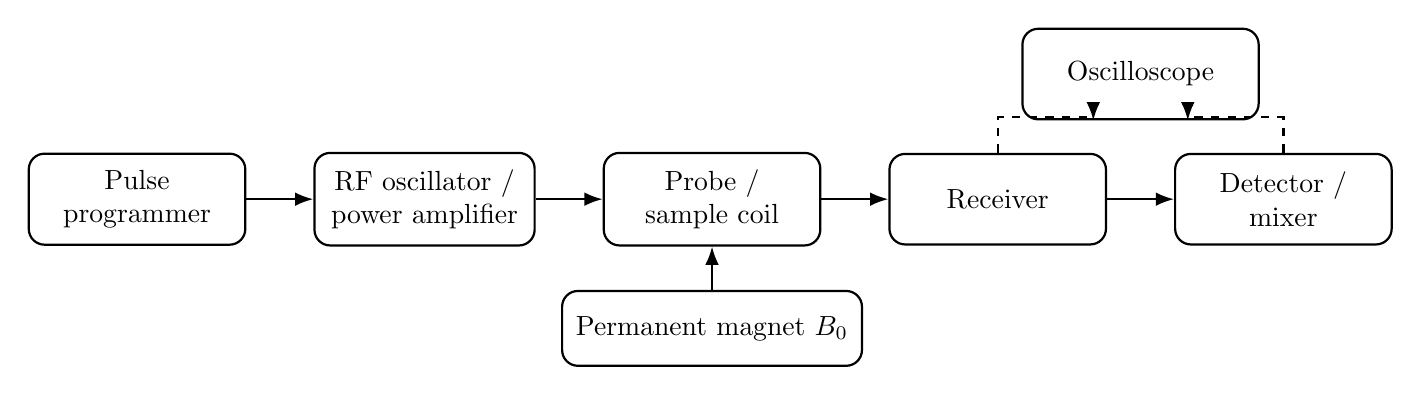
\begin{tikzpicture}[
    >=Latex,
    node distance=0.8cm and 0.85cm,
    block/.style={draw, rounded corners=2mm, thick, align=center, minimum height=1.15cm, minimum width=2.75cm, inner sep=6pt},
    smallblock/.style={draw, rounded corners=2mm, thick, align=center, minimum height=0.95cm, minimum width=2.45cm, inner sep=5pt},
    dashedlink/.style={->, thick, dashed},
    solidlink/.style={->, thick}
]
\node[block] (pp) {Pulse\\programmer};
\node[block, right=of pp] (rf) {RF oscillator /\\power amplifier};
\node[block, right=of rf] (probe) {Probe /\\sample coil};
\node[smallblock, below=0.55cm of probe] (mag) {Permanent magnet $B_0$};
\node[block, right=of probe] (recv) {Receiver};
\node[block, right=of recv] (det) {Detector /\\mixer};
\node[block, above=1.0cm of $(recv)!0.5!(det)$, minimum width=3.0cm] (scope) {Oscilloscope};

\draw[solidlink] (pp) -- (rf);
\draw[solidlink] (rf) -- (probe);
\draw[solidlink] (probe) -- (recv);
\draw[solidlink] (recv) -- (det);
\draw[solidlink] (mag.north) -- (probe.south);
\draw[dashedlink] (recv.north) -- ++(0,0.45) -| ($(scope.south)+(-0.6,0)$);
\draw[dashedlink] (det.north) -- ++(0,0.45) -| ($(scope.south)+(0.6,0)$);
\end{tikzpicture}
\caption{Functional apparatus chain used in the pulsed-NMR measurements. The main excitation and detection path is shown left-to-right. Dashed lines indicate that the oscilloscope monitored a selected receiver- or detector-stage output rather than lying in the main signal path.}
\label{fig:apparatus}
\end{figure}

\subsection{Pulse sequences and acquisition strategy}

Four pulse patterns were central to the experiment: a single approximately $\pi/2$ pulse for the FID, an inversion-recovery sequence $\pi - \tau - \pi/2$ for $T_1$, a two-pulse $\pi/2 - \tau - \pi$ sequence for a single spin echo, and a Meiboom-Gill multiple-echo sequence for $T_2$. These sequences are summarized in Fig.~\ref{fig:pulse}. The pulse widths were tuned empirically from the observed NMR response, not taken directly from the pulse-programmer cursor values. Resonance tuning and pulse calibration therefore controlled the quality of all subsequent measurements.

\begin{figure}[t]
\centering
\includegraphics[width=0.96\textwidth]{assets/figure2_pulse_sequences.pdf}
\caption{Pulse sequences used to generate the FID, inversion recovery, single-echo, and multiple-echo measurements.}
\label{fig:pulse}
\end{figure}

\subsection{Calibration, procedure, and uncertainty convention}

Before the NMR measurements, the pulse programmer was checked directly on the oscilloscope in single-pulse and two-pulse modes. These cursor readouts served as hardware sanity checks only; the final relaxation parameters were extracted from the NMR response itself. Mineral oil was then tuned to the zero-beat resonance condition, and the sample carriage was moved vertically and horizontally to locate the magnet ``sweet spot,'' defined operationally as the position at which the visible FID lasted longest.

For $T_1$, a rough repetition-time estimate was first used to establish the order of magnitude. The final inversion-recovery measurement employed a $\pi - \tau - \pi/2$ sequence in which the delay $\tau$ was scanned in \SI{5}{ms} increments and the baseline-subtracted detector amplitude was recorded. For $T_2$, the final quantitative value was taken from the Meiboom-Gill waveform export \texttt{DS0001A.CSV}. Positive echo maxima were detected after subtracting the pre-trigger baseline, and the resulting envelope was fit to a single exponential.

Uncertainties were assigned according to how the data were actually obtained. Cursor readouts from photographed scope screens were given practical uncertainties rather than the nominal least-significant digit of the display. In the inversion-recovery scan, the broad minimum and 5~ms delay step set the uncertainty in $\tau_0$. In the CSV-based $T_2$ fit, a per-peak amplitude uncertainty of \SI{1.3}{mV} was assigned by combining the measured baseline rms noise (\SI{0.89}{mV}) with an approximate \SI{1.0}{mV} peak-picking / quantization term in quadrature.

\section{Results}

Table~\ref{tab:summary} summarizes the principal reported quantities.

\begin{table}[t]
\centering
\caption{Summary of reported quantities.}
\label{tab:summary}
\begin{tabularx}{0.88\textwidth}{@{}L{0.52\textwidth}C{0.30\textwidth}@{}}
\toprule
\textbf{Quantity} & \textbf{Reported value} \\
\midrule
Mineral-oil zero-beat resonance & $f_0 \approx 15.146\ \mathrm{MHz}$ \\
Static magnetic field & $B_0 \approx 3.557\ \mathrm{kG}\ (0.3557\ \mathrm{T})$ \\
Approximate $\pi/2$ pulse width & $t_{\pi/2} \approx 8\ \mu\mathrm{s}$ \\
Approximate $\pi$ pulse width & $t_{\pi} \approx 18\ \mu\mathrm{s}$ \\
Pulse-width ratio & $t_{\pi}/t_{\pi/2} \approx 2.25$ \\
Spin-lattice relaxation time & $T_1 = (51 \pm 4)\ \mathrm{ms}$ \\
Spin-spin relaxation time & $T_2 = (45 \pm 3)\ \mathrm{ms}$ \\
\bottomrule
\end{tabularx}
\end{table}

\subsection{Pulse-programmer checks, resonance tuning, and sweet-spot search}

The pulse-programmer cursor checks confirmed that the A pulse had a finite width on the expected $10^{-5}$~s timescale and that the B pulse delay could be shifted reproducibly. These checks are summarized in Table~\ref{tab:partA}.

\begin{table}[H]
\centering
\caption{Part A quantitative cursor checks.}
\label{tab:partA}
\small
\begin{tabularx}{\textwidth}{@{}L{0.16\textwidth}L{0.26\textwidth}L{0.22\textwidth}Y@{}}
\toprule
\textbf{Trace} & \textbf{Approximate cursor values} & \textbf{Quantitative check} & \textbf{Interpretation} \\
\midrule
Single A pulse & $x_1 \approx -7.7\ \mu\mathrm{s},\ x_2 \approx 27.3\ \mu\mathrm{s}$ & $\Delta t \approx (35.1 \pm 1.0)\ \mu\mathrm{s}$ & Finite-width single pulse on the correct 10$^{-5}$ s timescale. \\
Two-pulse A/B sequence & $x_1 \approx 0.8\ \mu\mathrm{s},\ x_2 \approx 78.9\ \mu\mathrm{s}$ & $\Delta t \approx (78.2 \pm 1.0)\ \mu\mathrm{s}$ & The B pulse is delayed relative to the A pulse and the separation shifts reproducibly. \\
\bottomrule
\end{tabularx}
\end{table}

The mineral-oil resonance was found at the zero-beat condition near $f_0 \approx \SI{15.146}{MHz}$. Using the proton relation above, this corresponds to $B_0 \approx 3.557\,\mathrm{kG}$ ($\SI{0.3557}{T}$), essentially the nominal $3500\,\mathrm{G}$ field of the TeachSpin magnet.\cite{teachspin} The detector-out transient was longest at the sweet spot, where the field is most homogeneous and the spread of local Larmor frequencies is therefore smallest.

\begin{figure}[t]
\centering
\includegraphics[width=0.78\textwidth]{assets/figure3_fid_comparison.pdf}
\caption{Clean redrawing of the detector-out transient during the sweet-spot search. The curves were normalized and reconstructed from the observed scope traces to isolate the change in transient duration with sample position. The sweet-spot trace remains visible for longer times, consistent with improved field homogeneity and reduced dephasing.}
\label{fig:fid}
\end{figure}

\subsection{Inversion recovery and the extraction of $T_1$}

The final $T_1$ measurement used an inversion-recovery sequence. The pulse widths inferred from the NMR response were approximately $t_{\pi/2} \approx \SI{8}{\micro\second}$ and $t_\pi \approx \SI{18}{\micro\second}$, so the pulse-width ratio was about 2.25, reasonably close to the ideal factor of 2. For inversion recovery the longitudinal magnetization obeys
\[
M_z(\tau)=M_0\left[1-2e^{-\tau/T_1}\right],
\]
and the zero-crossing condition $M_z(\tau_0)=0$ gives
\[
T_1 = \frac{\tau_0}{\ln 2}.
\]
The notebook minimum occurred at $\tau_0 = \SI{35.5}{ms}$. Because the minimum was broad and the delay scan used \SI{5}{ms} steps, the practical uncertainty was taken as $\delta\tau_0 \approx \SI{2.5}{ms}$ rather than the much smaller formal display increment. The resulting example calculation is shown in Table~\ref{tab:t1calc}.

\begin{table}[H]
\centering
\caption{Example calculation and error propagation for $T_1$.}
\label{tab:t1calc}
\begin{tabularx}{0.88\textwidth}{@{}L{0.30\textwidth}Y@{}}
\toprule
\textbf{Measured quantity} & \textbf{Calculation} \\
\midrule
Zero-crossing delay & $\tau_0 = 35.5\ \mathrm{ms}$ \\
Central value & $T_1 = \tau_0/\ln 2 = 35.5/0.693 = 51.2\ \mathrm{ms}$ \\
Practical delay uncertainty & $\delta\tau_0 \approx 2.5\ \mathrm{ms}$, set by the 5 ms scan step and the broadness of the minimum \\
Error propagation & $\delta T_1 = \left|\partial T_1/\partial \tau_0\right|\,\delta\tau_0 = \delta\tau_0/\ln 2 = 2.5/0.693 = 3.6\ \mathrm{ms}$ \\
Reported result & $T_1 = (51 \pm 4)\ \mathrm{ms}$ \\
\bottomrule
\end{tabularx}
\end{table}

Figure~\ref{fig:t1} shows the baseline-subtracted inversion-recovery amplitudes together with a weighted nonlinear fit to the magnitude-detector model
\[
A(\tau) = A_{\mathrm{off}} + A_0\left|1 - 2e^{-\tau/T_1}\right|.
\]
The fit is used only as an internal consistency check, not as the primary reported value. It gives $T_1^{\mathrm{fit}} = (52.1 \pm 1.1)\,\si{ms}$, which agrees with the primary zero-crossing result $T_1 = (51 \pm 4)\,\si{ms}$ within uncertainty.

\begin{figure}[t]
\centering
\includegraphics[width=0.74\textwidth]{assets/figure4_t1_fit.pdf}
\caption{Baseline-subtracted inversion-recovery amplitudes for mineral oil. Open circles are the notebook data with practical $\pm \SI{5}{mV}$ amplitude uncertainties. The dashed curve is a weighted fit to the magnitude-detector model used only as a cross-check on the primary zero-crossing analysis.}
\label{fig:t1}
\end{figure}

\subsection{Spin echoes and the extraction of $T_2$}

A clear two-pulse spin echo was observed after the initial $\pi/2$ pulse, demonstrating that a substantial fraction of the apparent FID decay arose from reversible dephasing rather than irreversible relaxation. The final quantitative $T_2$ value was obtained from the exported Meiboom-Gill waveform \texttt{DS0001A.CSV}, not from a photographed scope screen. Table~\ref{tab:t2derived} lists the derived quantities used in the fit.

\begin{table}[H]
\centering
\caption{Derived quantities from the exported Meiboom-Gill waveform \texttt{DS0001A.CSV}.}
\label{tab:t2derived}
\begin{tabularx}{0.88\textwidth}{@{}L{0.40\textwidth}Y@{}}
\toprule
\textbf{CSV-derived quantity} & \textbf{Value} \\
\midrule
Memory length & 10 000 points \\
Sampling period & $10\ \mu\mathrm{s}$ \\
Pre-trigger baseline (median) & $118.0\ \mathrm{mV}$ \\
Baseline rms noise & $0.89\ \mathrm{mV}$ \\
Detected positive maxima & 36 \\
Assigned per-peak amplitude uncertainty & $\pm 1.3\ \mathrm{mV}$ \\
Exponential model & $A(t)=A_0 e^{-t/T_2}$ \\
Best-fit decay constant & $T_2^{\mathrm{fit}} = (44.7 \pm 1.0)\ \mathrm{ms}$ \\
Conservative reported value & $T_2 = (45 \pm 3)\ \mathrm{ms}$ \\
\bottomrule
\end{tabularx}
\end{table}

The waveform contained 10\,000 points sampled every \SI{10}{\micro\second}. A pre-trigger baseline of \SI{118.0}{mV} was estimated from the region $t<-\SI{5}{ms}$, and 36 positive echo maxima were then detected after the initial pulse ring-down. The echo envelope was fit to $A(t)=A_0 e^{-t/T_2}$, yielding $T_2^{\mathrm{fit}} = (44.7 \pm 1.0)\,\si{ms}$. To reflect reasonable baseline and peak-selection choices, the reported value is broadened conservatively to $T_2 = (45 \pm 3)\,\si{ms}$.

\begin{figure}[t]
\centering
\includegraphics[width=0.84\textwidth]{assets/figure5_t2_fit.pdf}
\caption{Formal extraction of $T_2$ from \texttt{DS0001A.CSV}. The upper panel shows the raw Meiboom-Gill waveform, the baseline estimate, and the detected maxima. The lower panel shows the baseline-subtracted echo envelope and the exponential fit $A(t)=A_0 e^{-t/T_2}$.}
\label{fig:t2}
\end{figure}

Figure~\ref{fig:cpmg} compares the multiple-echo behavior of the Carr-Purcell and Meiboom-Gill sequences without reproducing oscilloscope screenshots. The lower panel shows the actual normalized Meiboom-Gill maxima from \texttt{DS0001A.CSV}. The upper panel is a clean qualitative Carr-Purcell envelope drawn to match the faster, less stable decay observed during the scope comparison.

\begin{figure}[t]
\centering
\includegraphics[width=0.82\textwidth]{assets/figure6_cp_vs_mg.pdf}
\caption{Comparison of multiple-echo behavior. The Meiboom-Gill panel uses the normalized maxima extracted from \texttt{DS0001A.CSV}. The Carr-Purcell panel is a clean qualitative envelope that captures the faster and less stable decay seen during the oscilloscope comparison.}
\label{fig:cpmg}
\end{figure}

\subsection{Comparison of the principal observables and paraffin-wax follow-up}

The experiment probed three related but distinct time-domain observables. The single-pulse FID yielded an apparent decay dominated by reversible dephasing and therefore measured $T_2^\ast$ rather than the intrinsic $T_2$. Inversion recovery probed the recovery of $M_z$ and therefore isolated $T_1$. The Meiboom-Gill echo envelope suppressed static inhomogeneity and gave the cleanest route to $T_2$. These distinctions are summarized in Table~\ref{tab:comparison}.

\begin{table}[H]
\centering
\caption{Comparison of the main pulsed-NMR observables measured in this experiment.}
\label{tab:comparison}
\small
\begin{tabularx}{\textwidth}{@{}L{0.18\textwidth}L{0.19\textwidth}L{0.18\textwidth}L{0.19\textwidth}Y@{}}
\toprule
\textbf{Observable} & \textbf{How it was obtained} & \textbf{What it measures} & \textbf{Main limitation here} & \textbf{Takeaway} \\
\midrule
Observed FID decay ($T_2^\ast$) & Single approximately $\pi/2$ pulse on detector out & Loss of transverse phase coherence immediately after excitation & Strongly limited by field inhomogeneity and sweet-spot positioning & Position-dependent and not a direct measurement of the intrinsic $T_2$. \\
$T_1$ & $\pi - \tau - \pi/2$ inversion recovery & Recovery of longitudinal magnetization toward equilibrium & Delay-step granularity, pulse calibration, and resonance drift & Final reported value: $T_1 = (51 \pm 4)\ \mathrm{ms}$. \\
$T_2$ & Meiboom-Gill echo envelope from DS0001A.CSV & Irreversible transverse dephasing after static inhomogeneity is refocused & Baseline choice, peak-picking, diffusion, and residual pulse-angle errors & Final reported value: $T_2 = (45 \pm 3)\ \mathrm{ms}$. \\
\bottomrule
\end{tabularx}
\end{table}

A short follow-up also explored paraffin wax as it passed through solid, mixed, and liquid states under Meiboom-Gill conditions. The notes indicate that a strong, clean echo envelope was hardest to obtain in the mixed or partially molten state, consistent with the idea that sample heterogeneity and changing mobility complicate the relaxation behavior. Those observations were only qualitative and are not used in the quoted $T_1$ and $T_2$ values.

\section{Discussion}

The experiment reproduced the expected hierarchy of pulsed-NMR observables. The raw FID depended strongly on sample position and therefore reflected $T_2^\ast$ rather than the intrinsic $T_2$. The two-pulse echo showed that a significant part of the visible FID decay could be reversed, and the Meiboom-Gill echo train then yielded a robust transverse-relaxation value once an exported waveform was analyzed quantitatively.

The resonance result is particularly reassuring. The measured zero-beat frequency of \SI{15.146}{MHz} corresponds to $B_0 \approx 3.557\,\mathrm{kG}$, essentially the nominal $3500\,\mathrm{G}$ field of the TeachSpin magnet.\cite{teachspin} Likewise, the measured pulse-width ratio $t_\pi/t_{\pi/2} \approx 2.25$ is reasonably close to the ideal factor of 2. These agreements suggest that the RF tuning and basic pulse calibration were broadly correct before the relaxation measurements were attempted.

The largest quantitative tension in the dataset is the $T_1$ value. The inversion-recovery result $T_1 = (51 \pm 4)\,\si{ms}$ is substantially larger than the rough room-temperature guide often quoted for mineral oil in teaching materials (about \SI{12}{ms}).\cite{teachspin} Several factors can plausibly explain the discrepancy. First, the zero-crossing minimum is broad, so the practical uncertainty is controlled by the \SI{5}{ms} delay step rather than by the formal display resolution. Second, imperfect pulse calibration and slow resonance drift can shift the apparent minimum. Third, relaxation times in liquids depend on sample composition, viscosity, and temperature, so exact agreement with a handbook estimate is not expected.\cite{uwmanual} The independent weighted fit to the full inversion-recovery curve nevertheless agrees with the zero-crossing method, which shows that the reported $T_1$ does not depend on a single isolated point.

The $T_2$ result is stronger quantitatively because it was extracted from a digitally exported waveform rather than a photographed screen. Even so, the covariance of the exponential fit alone would understate the true uncertainty. The final $\pm \SI{3}{ms}$ uncertainty therefore includes practical effects from baseline choice, peak-picking, diffusion, and residual pulse-angle error. These uncertainties and concrete improvements are summarized in Table~\ref{tab:unc}.

\begin{table}[t]
\centering
\caption{Major uncertainties and concrete improvements.}
\label{tab:unc}
\small
\begin{tabularx}{\textwidth}{@{}L{0.22\textwidth}L{0.18\textwidth}L{0.24\textwidth}Y@{}}
\toprule
\textbf{Source of uncertainty} & \textbf{Most affected quantity} & \textbf{Likely effect} & \textbf{Improvement / mitigation} \\
\midrule
Resonance detuning and magnet drift & FID amplitude, pulse calibration, and both relaxation measurements & Detuning reduces the effective excitation and shifts the $\pi/2$ and $\pi$ conditions. & Retune the zero-beat condition before each scan and record the frequency setting whenever the sample is moved. \\
Sample position relative to the sweet spot & Observed FID lifetime ($T_2^\ast$) and echo quality & Field inhomogeneity broadens the resonance and shortens the visible FID. & Search for the longest-lived FID before each major acquisition and mark the optimized carriage position. \\
Finite delay steps near the inversion-recovery minimum & $T_1$ & A broad minimum means the zero crossing cannot be localized more precisely than a few milliseconds. & Repeat the scan with 1--2 ms steps near the minimum and average several traces at each point. \\
Peak selection and baseline choice in the CSV fit & $T_2$ & The fitted echo envelope shifts slightly if the baseline or peak windows are altered. & Use a consistent pre-trigger baseline definition and compare several reasonable peak-picking windows. \\
Pulse-angle errors in multiple-echo sequences & Especially CP; also residual effects in MG & Imperfect 180$^\circ$ refocusing makes the apparent decay faster, especially in the Carr-Purcell sequence. & Recalibrate the $\pi$ pulse carefully and prefer the Meiboom-Gill phase cycling for the final $T_2$ extraction. \\
Diffusion during the echo train & $T_2$ & Molecular motion through residual field gradients can make the measured decay slightly faster than the intrinsic spin-spin relaxation. & Use shorter echo spacings or a more homogeneous field when quantitative $T_2$ values are required. \\
\bottomrule
\end{tabularx}
\end{table}

Together, these observations show that the experiment was not simply a demonstration of oscilloscope operation. It was a controlled time-domain measurement in which pulse sequences were used to manipulate the spin system, isolate reversible and irreversible dephasing, and extract relaxation parameters that carry real physical meaning.

\section{Conclusion}

The pulsed-NMR experiment successfully demonstrated resonance tuning, free induction decay, spin-echo formation, inversion recovery, and extraction of the relaxation parameters $T_1$ and $T_2$ from time-domain measurements. Mineral oil resonated near $f_0 \approx \SI{15.146}{MHz}$, corresponding to $B_0 \approx 3.557\,\mathrm{kG}$. The primary inversion-recovery analysis gave $T_1 = (51 \pm 4)\,\si{ms}$, and a weighted nonlinear cross-check gave $T_1^{\mathrm{fit}} = (52.1 \pm 1.1)\,\si{ms}$. The Meiboom-Gill waveform export yielded $T_2^{\mathrm{fit}} = (44.7 \pm 1.0)\,\si{ms}$ and a conservative reported value $T_2 = (45 \pm 3)\,\si{ms}$. The main limitations were resonance drift, finite delay steps near the inversion-recovery minimum, field inhomogeneity, and practical peak-selection uncertainty in the echo train, but the overall results remain physically consistent with the expected distinction between $T_2^\ast$, $T_1$, and $T_2$.

\section*{Supplementary submission files}
The raw notebook export (\texttt{PNMR Lab.pdf}) and the exported waveform file (\texttt{DS0001A.CSV}) are intended to accompany this report as supplementary submission files.

\begin{thebibliography}{9}
\bibitem{teachspin}
TeachSpin, Inc., \emph{Pulsed Nuclear Magnetic Resonance Spectrometer PS1-A Manual}.

\bibitem{uwmanual}
University of Washington, \emph{Pulsed Nuclear Magnetic Resonance Laboratory Manual}.

\bibitem{preston}
D. W. Preston and E. R. Dietz, ``Introduction to Magnetic Resonance,'' in \emph{The Art of Experimental Physics}, pp. 264--272.
\end{thebibliography}

\appendix

\section{Raw inversion-recovery data}

\begin{table}[H]
\centering
\caption{Raw inversion-recovery data recorded in the notebook.}
\label{tab:rawt1}
\begin{tabular}{@{}rrrr@{}}
\toprule
\textbf{Delay $\tau$ (ms)} & \textbf{Measured peak (mV)} & \textbf{Baseline (mV)} & \textbf{Amplitude above baseline (mV)} \\
\midrule
10 & 175 $\pm$ 5 & 90 & 85 $\pm$ 5 \\
15 & 158 $\pm$ 5 & 90 & 68 $\pm$ 5 \\
20 & 143 $\pm$ 5 & 90 & 53 $\pm$ 5 \\
25 & 132 $\pm$ 5 & 90 & 42 $\pm$ 5 \\
30 & 124 $\pm$ 5 & 90 & 34 $\pm$ 5 \\
35 & 120 $\pm$ 5 & 90 & 30 $\pm$ 5 \\
40 & 120 $\pm$ 5 & 90 & 30 $\pm$ 5 \\
45 & 125 $\pm$ 5 & 90 & 35 $\pm$ 5 \\
50 & 130 $\pm$ 5 & 90 & 40 $\pm$ 5 \\
55 & 136 $\pm$ 5 & 90 & 46 $\pm$ 5 \\
60 & 143 $\pm$ 5 & 90 & 53 $\pm$ 5 \\
65 & 150 $\pm$ 5 & 90 & 60 $\pm$ 5 \\
70 & 158 $\pm$ 5 & 90 & 68 $\pm$ 5 \\
75 & 170 $\pm$ 5 & 90 & 80 $\pm$ 5 \\
80 & 182 $\pm$ 5 & 90 & 92 $\pm$ 5 \\
\bottomrule
\end{tabular}
\end{table}

\section{Echo maxima used in the $T_2$ fit}

\small
\begin{longtable}{@{}rrrrr@{}}
\caption{Echo maxima extracted from \texttt{DS0001A.CSV}. Each baseline-subtracted amplitude carries an assigned $1\sigma$ uncertainty of $\pm \SI{1.3}{mV}$, obtained by combining the pre-trigger baseline rms noise (\SI{0.89}{mV}) with an approximate \SI{1.0}{mV} peak-picking / quantization term in quadrature.}\label{tab:maxtable}\\
\toprule
\textbf{\#} & \textbf{$t$ (ms)} & \textbf{Peak (mV)} & \textbf{$A$ above baseline (mV)} & \textbf{$\sigma_A$ (mV)} \\
\midrule
\endfirsthead

\toprule
\textbf{\#} & \textbf{$t$ (ms)} & \textbf{Peak (mV)} & \textbf{$A$ above baseline (mV)} & \textbf{$\sigma_A$ (mV)} \\
\midrule
\endhead

\midrule
\multicolumn{5}{r}{Continued on next page}\\
\endfoot

\bottomrule
\endlastfoot
1 & 0.98 & 166.0 & 48.0 & 1.3 \\
2 & 3.02 & 164.0 & 46.0 & 1.3 \\
3 & 5.05 & 160.0 & 42.0 & 1.3 \\
4 & 6.97 & 158.0 & 40.0 & 1.3 \\
5 & 9.04 & 152.0 & 34.0 & 1.3 \\
6 & 11.04 & 156.0 & 38.0 & 1.3 \\
7 & 13.01 & 150.0 & 32.0 & 1.3 \\
8 & 14.99 & 152.0 & 34.0 & 1.3 \\
9 & 17.00 & 150.0 & 32.0 & 1.3 \\
10 & 18.97 & 150.0 & 32.0 & 1.3 \\
11 & 21.03 & 146.0 & 28.0 & 1.3 \\
12 & 23.00 & 144.0 & 26.0 & 1.3 \\
13 & 25.04 & 142.0 & 24.0 & 1.3 \\
14 & 26.96 & 146.0 & 28.0 & 1.3 \\
15 & 29.03 & 142.0 & 24.0 & 1.3 \\
16 & 30.97 & 142.0 & 24.0 & 1.3 \\
17 & 33.03 & 140.0 & 22.0 & 1.3 \\
18 & 34.97 & 140.0 & 22.0 & 1.3 \\
19 & 36.99 & 138.0 & 20.0 & 1.3 \\
20 & 38.98 & 138.0 & 20.0 & 1.3 \\
21 & 41.07 & 134.0 & 16.0 & 1.3 \\
22 & 42.98 & 136.0 & 18.0 & 1.3 \\
23 & 45.01 & 136.0 & 18.0 & 1.3 \\
24 & 47.00 & 136.0 & 18.0 & 1.3 \\
25 & 49.05 & 132.0 & 14.0 & 1.3 \\
26 & 50.99 & 134.0 & 16.0 & 1.3 \\
27 & 53.04 & 130.0 & 12.0 & 1.3 \\
28 & 55.08 & 130.0 & 12.0 & 1.3 \\
29 & 57.00 & 132.0 & 14.0 & 1.3 \\
30 & 59.01 & 134.0 & 16.0 & 1.3 \\
31 & 60.99 & 130.0 & 12.0 & 1.3 \\
32 & 62.96 & 130.0 & 12.0 & 1.3 \\
33 & 64.98 & 130.0 & 12.0 & 1.3 \\
34 & 67.02 & 130.0 & 12.0 & 1.3 \\
35 & 69.02 & 128.0 & 10.0 & 1.3 \\
36 & 71.00 & 128.0 & 10.0 & 1.3 \\
\end{longtable}

\end{document}
